% Options for packages loaded elsewhere
\PassOptionsToPackage{unicode}{hyperref}
\PassOptionsToPackage{hyphens}{url}
\documentclass[
  10pt,
  a4paper,
]{article}
\usepackage{xcolor}
\usepackage[margin=22mm]{geometry}
\usepackage{amsmath,amssymb}
\setcounter{secnumdepth}{-\maxdimen} % remove section numbering
\usepackage{iftex}
\ifPDFTeX
  \usepackage[T1]{fontenc}
  \usepackage[utf8]{inputenc}
  \usepackage{textcomp} % provide euro and other symbols
\else % if luatex or xetex
  \usepackage{unicode-math} % this also loads fontspec
  \defaultfontfeatures{Scale=MatchLowercase}
  \defaultfontfeatures[\rmfamily]{Ligatures=TeX,Scale=1}
\fi
\usepackage{lmodern}
\ifPDFTeX\else
  % xetex/luatex font selection
\fi
% Use upquote if available, for straight quotes in verbatim environments
\IfFileExists{upquote.sty}{\usepackage{upquote}}{}
\IfFileExists{microtype.sty}{% use microtype if available
  \usepackage[]{microtype}
  \UseMicrotypeSet[protrusion]{basicmath} % disable protrusion for tt fonts
}{}
\makeatletter
\@ifundefined{KOMAClassName}{% if non-KOMA class
  \IfFileExists{parskip.sty}{%
    \usepackage{parskip}
  }{% else
    \setlength{\parindent}{0pt}
    \setlength{\parskip}{6pt plus 2pt minus 1pt}}
}{% if KOMA class
  \KOMAoptions{parskip=half}}
\makeatother
\usepackage{graphicx}
\makeatletter
\newsavebox\pandoc@box
\newcommand*\pandocbounded[1]{% scales image to fit in text height/width
  \sbox\pandoc@box{#1}%
  \Gscale@div\@tempa{\textheight}{\dimexpr\ht\pandoc@box+\dp\pandoc@box\relax}%
  \Gscale@div\@tempb{\linewidth}{\wd\pandoc@box}%
  \ifdim\@tempb\p@<\@tempa\p@\let\@tempa\@tempb\fi% select the smaller of both
  \ifdim\@tempa\p@<\p@\scalebox{\@tempa}{\usebox\pandoc@box}%
  \else\usebox{\pandoc@box}%
  \fi%
}
% Set default figure placement to htbp
\def\fps@figure{htbp}
\makeatother
\setlength{\emergencystretch}{3em} % prevent overfull lines
\providecommand{\tightlist}{%
  \setlength{\itemsep}{0pt}\setlength{\parskip}{0pt}}
\usepackage{mathrsfs}
\newcommand{\Log}{\operatorname{Log}}
\usepackage{mathtools}
\usepackage{xurl}
\emergencystretch=3em
\setcounter{tocdepth}{1}
\newcommand{\Beta}{\mathrm{B}}
\DeclareUnicodeCharacter{00B2}{\ensuremath{^2}}
\DeclareUnicodeCharacter{00B1}{\ensuremath{\pm}}
\DeclareUnicodeCharacter{00D7}{\ensuremath{\times}}
\DeclareUnicodeCharacter{2192}{\ensuremath{\to}}
\DeclareUnicodeCharacter{21D2}{\ensuremath{\Rightarrow}}
\DeclareUnicodeCharacter{21A6}{\ensuremath{\mapsto}}
\DeclareUnicodeCharacter{2208}{\ensuremath{\in}}
\DeclareUnicodeCharacter{2209}{\ensuremath{\notin}}
\DeclareUnicodeCharacter{2212}{\ensuremath{-}}
\DeclareUnicodeCharacter{2227}{\ensuremath{\wedge}}
\DeclareUnicodeCharacter{2228}{\ensuremath{\vee}}
\DeclareUnicodeCharacter{2260}{\ensuremath{\ne}}
\DeclareUnicodeCharacter{2264}{\ensuremath{\le}}
\DeclareUnicodeCharacter{2265}{\ensuremath{\ge}}
\DeclareUnicodeCharacter{2297}{\ensuremath{\otimes}}
\DeclareUnicodeCharacter{00B3}{\ensuremath{^3}}
\DeclareUnicodeCharacter{2074}{\ensuremath{^4}}
\DeclareUnicodeCharacter{2076}{\ensuremath{^6}}
\DeclareUnicodeCharacter{03BB}{\ensuremath{\lambda}}
\DeclareUnicodeCharacter{03BC}{\ensuremath{\mu}}
\DeclareUnicodeCharacter{03B5}{\ensuremath{\epsilon}}
\DeclareUnicodeCharacter{03C4}{\ensuremath{\tau}}
\DeclareUnicodeCharacter{03A6}{\ensuremath{\Phi}}
\DeclareUnicodeCharacter{03B1}{\ensuremath{\alpha}}
\DeclareUnicodeCharacter{03C3}{\ensuremath{\sigma}}
\DeclareUnicodeCharacter{03B4}{\ensuremath{\delta}}
\DeclareUnicodeCharacter{03C0}{\ensuremath{\pi}}
\DeclareUnicodeCharacter{039B}{\ensuremath{\Lambda}}
\DeclareUnicodeCharacter{2202}{\ensuremath{\partial}}
\DeclareUnicodeCharacter{0393}{\ensuremath{\Gamma}}
\DeclareUnicodeCharacter{2205}{\ensuremath{\varnothing}}
\DeclareUnicodeCharacter{221E}{\ensuremath{\infty}}
\DeclareUnicodeCharacter{2200}{\ensuremath{\forall}}
\DeclareUnicodeCharacter{00B9}{\ensuremath{^1}}
\DeclareUnicodeCharacter{00B0}{\ensuremath{{}^\circ}}
\DeclareUnicodeCharacter{211D}{\ensuremath{\mathbb{R}}}
\usepackage{bookmark}
\IfFileExists{xurl.sty}{\usepackage{xurl}}{} % add URL line breaks if available
\urlstyle{same}
\hypersetup{
  hidelinks,
  pdfcreator={LaTeX via pandoc}}

\author{}
\date{}

\begin{document}

{
\setcounter{tocdepth}{3}
\tableofcontents
}
\section{From the signed cover to an arithmetic quadratic
cover}\label{from-the-signed-cover-to-an-arithmetic-quadratic-cover}

This calculation uses Alain Connes and Caterina Consani,
\href{https://arxiv.org/abs/2501.06560v1}{Knots, primes and class field
theory, arXiv:2501.06560v1}, introductory Theorem 1 and the source
labels \texttt{coverdef}, \texttt{mappingtorus1}, \texttt{artinrec}, and
\texttt{main}. The original author TeX, rather than a PDF, was read
through its entire body and bibliography. Their theorem supplies the
arithmetic cover and its Frobenius monodromy. The calculations below
specify the quotient of the programme's signed cover which enters that
theorem, and the infinitesimal information its quotient forgets.

The incoming monodromy and collision proofs are
\href{https://github.com/KokunoYumeto/zeta-function-research-reader/blob/adfbfe74fa49e31cb7aa068cf755fb083be37c32/workbenches/splitzero-tandem/branches/tau-zero-prime-positivity/EIGHT_STATE_HOLONOMY_DERIVATION.md}{EHM1--EHM53}.
The original order-192 group is the prior programme result
\href{https://github.com/KokunoYumeto/zeta-function-research-reader/blob/ab45e221579a0d48ce2885b4ecdf1a6aefc24a20/workbenches/splitzero-tandem/continuations/20260920-fable-boundary-action/FABLE_TO_ORIGINAL_CONDUCTOR.tex\#L2097}{SM1--SM19,
source lines 2097--2513}. Its abelian quotient is computed here; no
novelty is claimed for quadratic fields, discriminants, or Gauss sums.

\subsection{1. The exact abelian
quotient}\label{the-exact-abelian-quotient}

Write the full signed permutation group in its original convention as \[
G=\{(\sigma,\pi):\sigma\in\{1,-1\}^4,\ \pi\in S_4,
\ \prod_j\sigma_j=\operatorname{sgn}\pi\}.
\tag{CBR1}
\] It acts on the eight states \((j,\epsilon)\), with one pair over each
of the four roots, by signed permutations. It has order
\(8\cdot24=192\). Let \[
N=\{(\sigma,1):\prod_j\sigma_j=1\},\qquad
\chi_{\mathrm{disc}}(\sigma,\pi)=\operatorname{sgn}\pi.
\tag{CBR2}
\] Projection to \(S_4\) is onto: choose any sign vector whose product
is the required parity. Its kernel is \(N\).

We have the exact calculation \[
[G,G]=\{(\sigma,\pi):\pi\in A_4,\ \prod_j\sigma_j=1\},
\qquad G^{\mathrm{ab}}\cong\{1,-1\}
\tag{CBR3}
\] with quotient map \(\chi_{\mathrm{disc}}\). Here is a proof retaining
the kernel. Identify \(N\) with the even-coordinate-sum subspace of
\(\mathbb F_2^4\). Conjugation by any lift of \(\pi\) permutes its
coordinates. Given distinct \(a,b,c\), take \(v=e_a+e_b\) and
\(\pi=(b\ c)\). The commutator of a lift of \(\pi\) with \(v\) is
\(\pi v-v=e_b+e_c\). These pair vectors span all of \(N\), so
\(N\subseteq[G,G]\). The derived subgroup maps onto \([S_4,S_4]=A_4\):
the sign kills commutators, and the commutators of two transpositions
sharing one letter are three-cycles; three-cycles generate \(A_4\). The
latter generation follows by splitting every even-length word in
transpositions into pairs, and writing two disjoint transpositions as a
product of two three-cycles. Thus the derived subgroup contains the
entire preimage of \(A_4\), and containment in the reverse direction
follows from the sign homomorphism. This proves (CBR3), including its
order 96 and its universal property for homomorphisms from \(G\) into
abelian groups.

There is a different quotient on the original set of eight points. The
subgroup \([G,G]\) is transitive on it: an even permutation moves a
chosen root label to any other root label, and an even sign change
involving that root and one other root prescribes its sign. Hence \[
\{\text{eight states}\}/[G,G]=\{*\}.
\tag{CBR4}
\] Any equivariant map of the eight-point set into a set on which the
action factors through an abelian group therefore has singleton image.
In contrast, the regular frame torsor of \(G\) has the two-point
quotient \(G/[G,G]\). The double cover below is a quotient of this frame
cover, not an unidentified double quotient of the eight individual
states. Equations (CBR3) and (CBR4) prove the exact relation and the
distinct kernels.

There is also an explicit common finite cover retaining both objects.
Let \(H\) stabilize the state \((1,+)\), and let \(D_G=[G,G]\). Then
\(|H|=24\). The restriction of \(\chi_{\mathrm{disc}}\) to \(H\) is
onto: a transposition of two other root labels, together with a sign
change at a third other root, fixes \((1,+)\) and has character \(-1\).
Hence \(|H\cap D_G|=12\), and \[
G/(H\cap D_G)\xrightarrow{\ \sim\ }
(G/H)\times(G/D_G),\qquad
g(H\cap D_G)\longmapsto(gH,gD_G).
\tag{CBR4a}
\] It is injective by the intersection of the stabilizers. To hit a
prescribed pair, first choose the desired \(gH\), then multiply \(g\) on
the right by an element of \(H\) with the required sign; this adjusts
the second coordinate without changing the first. This proves
surjectivity and equivariance. Projection to the eight-state factor has
two-point fibres; projection to the character factor has eight-point
fibres. Applied to the frame torsor over the discriminant complement,
the same equivariant maps give its associated degree-16 cover and the
two covering maps. Thus the failed double quotient of the eight states
instead determines a common cover with completely specified maps.

\subsection{2. The discriminant in the original
coefficients}\label{the-discriminant-in-the-original-coefficients}

The polynomial in the original affine chart is \[
F(R)=AR^4+R^3+BR^2+CR+D.
\tag{CBR5}
\] On \(A\ne0\) with distinct roots \(R_1,\ldots,R_4\), put
\(\Delta=\prod_{i<j}(R_i-R_j)\) and \(\mathfrak D=A^6\Delta^2\). This
discriminant is a polynomial in the coefficients and extends to the
binary-quartic chart with a root at infinity. On the frame cover choose
the component whose derivative square roots satisfy \[
T_j^2=F'(R_j),\qquad
w=A^3\Delta=A\prod_{j=1}^4T_j,\qquad w^2=\mathfrak D.
\tag{CBR6}
\] Indeed \(\prod_jF'(R_j)=A^4\Delta^2\): each unordered root pair
contributes a minus sign, and there are six pairs. Thus the ratio of the
two candidate square roots in (CBR6) is a constant sign; the component
choice sets it to one. Under a signed permutation, \(\Delta\) changes by
\(\operatorname{sgn}\pi\), and \(\prod T_j\) changes by
\(\prod\sigma_j\). These agree exactly by (CBR1). Consequently the
double cover \[
w^2=\mathfrak D
\tag{CBR7}
\] is the character quotient (CBR3). On the discriminant complement its
derivative with respect to \(w\) is nonzero, so it is an unramified
double cover. The reciprocal chart of EHM1--EHM5 retains this cover at
\(A=0\); the value of \(\mathfrak D\) does not require dividing by
\(A\).

Along the original infinity path \((A,B,C,D)=(A,0,-1,0)\), \[
F(R)=R(AR^3+R^2-1),\qquad
\mathfrak D=4-27A^2.
\tag{CBR8}
\] The product discriminant identity gives the cubic discriminant
because the resultant with \(R\) is \(-1\), whose square is one.
Substituting \(a=A,b=1,c=0,d=-1\) into the cubic discriminant, or
eliminating the common root of the cubic and its derivative, gives
\(4-27A^2\). At the rational parameter \(A=1\), (CBR7) is the field \[
K=\mathbb Q[w]/(w^2+23).
\tag{CBR9}
\] The polynomial is irreducible over \(\mathbb Q\), since a rational
square cannot be negative. This is a specialization of the double-cover
equation, not an assertion that the full geometric order-192 monodromy
specializes unchanged to an arithmetic Galois group.

\subsection{3. An explicit map into the class-field
cover}\label{an-explicit-map-into-the-class-field-cover}

Let \(\zeta=e^{2\pi i/23}\), and let \(\lambda(a)\) be the quadratic
character of \(\mathbb F_{23}^{\times}\), extended by zero at zero. Its
square residues are \[
1,2,3,4,6,8,9,12,13,16,18.
\tag{CBR10}
\] These are the squares of \(1,\ldots,11\) modulo 23, so exactly eleven
nonzero elements are squares, and \(-1\) is not. Multiplication by a
nonsquare exchanges the two cosets of the subgroup of squares, proving
\(\sum_{a\ne0}\lambda(a)=0\). Define \[
\tau_{23}=\sum_{a=1}^{22}\lambda(a)\zeta^a.
\tag{CBR11}
\] Conjugation gives \(\overline{\tau}_{23}=-\tau_{23}\). Directly, \[
|\tau_{23}|^2
=\sum_{t\ne0}\lambda(t)\sum_{b\ne0}\zeta^{(t-1)b}
=22-\sum_{t\ne1}\lambda(t)=23.
\tag{CBR12}
\] The inner sum is 22 for \(t=1\) and \(-1\) otherwise, by the
geometric sum for the 23rd roots of unity. Therefore
\(\tau_{23}^2=-23\), and \[
K\xrightarrow{\ \sim\ }\mathbb Q(\tau_{23})\subset\mathbb Q(\zeta),
\qquad w\longmapsto\tau_{23}
\tag{CBR13}
\] is a field isomorphism onto its image. The polynomial
\(1+X+\cdots+X^{22}\) is irreducible by Eisenstein after
\(X\mapsto X+1\); thus all substitutions \(\zeta\mapsto\zeta^r\),
\(r\in\mathbb F_{23}^{\times}\), are the cyclotomic automorphisms.
Reindexing the finite sum gives \[
\sigma_r(\tau_{23})=\lambda(r)\tau_{23}.
\tag{CBR14}
\] This proves the arithmetic character without inferring it solely from
the degree of the field.

In the notation of Connes--Consani the required continuous surjection is
\[
\chi_{23}:\widehat{\mathbb Z}^{\times}\twoheadrightarrow\{1,-1\},
\qquad u\longmapsto\lambda(u_{23}\bmod23).
\tag{CBR15}
\] It is onto by (CBR10), trivial at every other local unit factor, and
factors at 23 through reduction modulo 23. It does not factor through
the trivial unit quotient, so its conductor is exactly 23. Equations
(CBR13)--(CBR15), followed by the source's Artin map, identify its field
with (CBR9).

For every prime \(p\ne23\), the source theorem now supplies the precise
periodic return \[
\operatorname{Mon}(C_p)=\lambda(p),\qquad |C_p|=\log p.
\tag{CBR16}
\] In particular \(p=2\) has two separate lifted circles, each of length
\(\log2\), and \(p=5\) has one circle of length \(2\log5\). At 23 the
quadratic character is ramified. These assertions follow by following
multiplication by \(+1\) or \(-1\) on the two-element fibre, not by
treating the sign as a positive or negative norm.

The integral model at 2 matters. Put \(\theta=(1+w)/2\). Then \[
\theta^2-\theta+6=0,\qquad
\mathbb Z[w]\subset\mathbb Z[\theta],\qquad
\mathbb Z[\theta]/\mathbb Z[w]\cong\mathbb Z/2.
\tag{CBR17}
\] Both modules have basis \((1,w)\) or \((1,\theta)\), and
\(w=2\theta-1\), proving the index. In fact \(\mathbb Z[\theta]\) is the
full ring of integers: an integral \(x=a+bw\) has trace
\(m=2a\in\mathbb Z\) and norm \(a^2+23b^2\in\mathbb Z\). Hence
\(23(2b)^2\in\mathbb Z\). If \(2b=r/s\) in lowest terms, \(s^2\mid23\),
forcing \(s=1\); write \(2b=n\in\mathbb Z\). Norm integrality then says
\(m^2+23n^2\equiv0\pmod4\), so \(m,n\) have the same parity. Thus
\(x=(m-n)/2+n\theta\in\mathbb Z[\theta]\). Conversely this ring is
integral by the displayed monic polynomial. Its two exact reductions are
\[
\mathbb Z[w]/2\cong\mathbb F_2[\eta]/(\eta^2),\quad\eta=w+1;
\qquad
\mathbb Z[\theta]/2\cong\mathbb F_2\times\mathbb F_2.
\tag{CBR18}
\] The second isomorphism is evaluation at \(\theta=0,1\), since the
defining polynomial reduces to \(\theta(\theta-1)\). It is the maximal
order which records the unramified split prime 2. The nonzero nilpotent
of the first reduction records the nonmaximal order and must not be used
to assign ramification to the field cover.

\subsection{4. The heat collision retains more than this
character}\label{the-heat-collision-retains-more-than-this-character}

On the actual heat path of EHM23, \[
F_h(R)=(R-1)(R^2+R-16h),\qquad
\mathfrak D(h)=(2-16h)^2(1+64h).
\tag{CBR19}
\] For a direct calculation, the quadratic discriminant is \(1+64h\),
and its resultant with \(R-1\) is its value \(2-16h\) at 1. Put
\(t=h-1/8\). The pulled-back double-cover ring over convergent complex
germs is \[
B=\mathbb C\{t\}[w]/\bigl(w^2-256t^2(9+64t)\bigr).
\tag{CBR20}
\] Choose the analytic square root \(a(t)=\sqrt{9+64t}\) with
\(a(0)=3\); its convergent binomial series specifies the branch. Define
\[
B\hookrightarrow\widetilde B=\mathbb C\{t\}\oplus\mathbb C\{t\},
\qquad f(t)+g(t)w\longmapsto
\bigl(f+16ta(t)g,\ f-16ta(t)g\bigr).
\tag{CBR21}
\] The map respects the relation, is injective, and its image consists
exactly of pairs whose difference lies in \(t\mathbb C\{t\}\). Indeed
the inverse expressions are \(f=(x+y)/2\) and \(g=(x-y)/(32ta(t))\).
Thus \[
\widetilde B/B\cong\mathbb C,\qquad
(x,y)\longmapsto (x-y)\bmod t.
\tag{CBR22}
\] The product ring is the integral closure of \(B\) in its total
quotient ring. To see this, its idempotent \((1,0)\) is integral, and
adjoining it to the diagonal germ ring produces all of \(\widetilde B\);
each convergent germ ring is a discrete valuation ring and hence
integrally closed. An element integral over \(B\) in either fraction
component is integral over the corresponding germ ring after projection,
so belongs to that ring. This proves both containments. Its conductor
back into \(B\) is \(t\widetilde B\): multiplying by the two component
idempotents tests that both coordinates vanish modulo \(t\).

The special fibres and the induced map are \[
B/tB=\mathbb C[w]/(w^2)
\longrightarrow\widetilde B/t\widetilde B=\mathbb C\oplus\mathbb C,
\qquad c+dw\longmapsto(c,c).
\tag{CBR23}
\] Its kernel is \(\mathbb Cw\), and its cokernel is the difference
line. These facts do not contradict injectivity before taking the fibre:
tensoring the exact sequence in (CBR22) with \(\mathbb C\{t\}/(t)\)
gives the connecting isomorphism from its \(\operatorname{Tor}_1\) to
that kernel. Explicitly the free resolution with differential
multiplication by \(t\) computes
\(\operatorname{Tor}_1(\mathbb C,\mathbb C)=\mathbb C\); exactness or
lifting a difference representative yields the nonzero kernel line. The
dual-number collision and its two separate normalized points are both
retained by (CBR21)--(CBR23).

On a punctured disk at \(h=1/8\) the character cover is trivial: its two
sheets are the analytic graphs \(w=\pm16ta(t)\). The zero of the
discriminant has order two and its square root has no branch monodromy
there. At \(h=-1/64\), the factor \(1+64h\) has a simple zero and
\(2-16h\ne0\), so the two sheets are exchanged. On the signed-cover
group this agrees exactly with \[
\chi_{\mathrm{disc}}(g_c)=+1,\qquad
\chi_{\mathrm{disc}}(g_d)=-1,\qquad
\chi_{\mathrm{disc}}(g_d^2)=+1.
\tag{CBR24}
\] Indeed \(g_c\) changes signs in two root pairs without permuting
roots; \(g_d\) interchanges two root labels; and its square again has
trivial root permutation, using the explicitly based loops EHM25.

The original full collision algebra is the different algebra \[
\mathscr L_0=\mathbb C[T]/(T^4),\qquad
\mathfrak N=(T),\qquad
\mathscr L_0/\mathfrak N^2\cong\mathbb C[\epsilon]/(\epsilon^2),
\quad \epsilon\longleftrightarrow T\bmod T^2.
\tag{CBR25}
\] One explicit isomorphism from the double-cover special fibre (CBR23)
to this last quotient sends \(w\) to \(T\bmod T^2\). This is an
isomorphism of the displayed complex algebras, with zero kernel and
inverse determined by \(T\bmod T^2\mapsto w\). It is not the fibre of
the normalization map (CBR21), whose kernel is nonzero. No
identification of the two families or of their monodromy actions follows
from this special-fibre isomorphism.

The based transport \(g_d^2\), invisible to (CBR24), has the nonzero
operator residue proved in EHM43--EHM46: \[
\delta=-\frac{T^3}{16}\frac{d}{dT},\qquad
\delta(T)=-\frac{T^3}{16},\quad
\delta(1)=\delta(T^2)=\delta(T^3)=0.
\tag{CBR26}
\] The derivation is well defined modulo \(T^4\) because it sends
\(T^4\) to a multiple of \(T^6\); it is nonzero and has square zero. In
the original generators \[
n_1=T^2/2,\quad n_2=3T+T^3/6,\quad n_3=T^3/2,
\qquad
\delta:\mathfrak N/\mathfrak N^2\xrightarrow{\ \sim\ }\mathfrak N^3,
\quad[n_2]\longmapsto-3n_3/8.
\tag{CBR27}
\] Each space is one-dimensional and the displayed coefficient is
nonzero. In particular the vanishing character monodromy in (CBR24)
coexists with a nonzero map between infinitesimal layers. Neither
averaging the quadratic character nor passing to the normalized
two-sheet fibre retains this map automatically.

\subsection{5. The trace map into the supported-zero
programme}\label{the-trace-map-into-the-supported-zero-programme}

The oriented periodic trace, including inertia invariants and both
traversals, is proved in
\href{https://github.com/KokunoYumeto/zeta-function-research-reader/blob/4a4238afc992e77aee83b97d38a1a63d283f540c/workbenches/splitzero-tandem/branches/tau-zero-prime-positivity/PRIME_HOLONOMY_SUPPORTED_WEIL_DERIVATION.md}{PHW1--PHW22}.
For the quadratic character (CBR15), it specializes to the finite
distribution on a compactly supported smooth test \(h\) \[
P_{\lambda}(h)=\sum_{p\ne23}\sum_{k\ge1}
(\log p)p^{-k/2}\lambda(p)^k
\bigl(h(-k\log p)+h(k\log p)\bigr).
\tag{CBR28}
\] If the support is in \([-R,R]\), only \(k\log p\le R\) contribute.
For \(p=5\), odd iterates carry coefficient \(-1\) and even iterates
coefficient \(+1\); for \(p=2\), all carry \(+1\). These are actual
powers of Frobenius, not a choice to replace a negative trace by its
absolute value.

For the two-dimensional regular representation of \(\{1,-1\}\), the
exact character decomposition is \(\mathbb C\oplus\mathbb C_\lambda\).
Therefore its periodic distribution is \(P_{\mathrm{fin}}+P_\lambda\);
at 23 only its trivial line survives the inertia projection. At every
separate supported or unsupported global zero, the coefficient space is
instead the single trivial line, since the full compact unit group fixes
that carrier point. The projector is \[
P_0=\tfrac12(I+\rho(-1)),\qquad
\operatorname{im}P_0=\mathbb C,\quad
\ker P_0=\mathbb C_\lambda.
\tag{CBR29}
\] In the group-ring trace of PHW17, augmentation has exactly this
trivial-character observation. It returns the complete supported-zero
formula
\href{https://github.com/KokunoYumeto/zeta-function-research-reader/blob/adfbfe74fa49e31cb7aa068cf755fb083be37c32/workbenches/splitzero-tandem/branches/tau-zero-prime-positivity/SUPPORTED_ZERO_PRIME_WEIL_DERIVATION.md}{SZW33--SZW42},
with the separate fixed-support labels and Fourier partners. The
complementary character retains (CBR28). Thus the arithmetic quotient
has a defined map to the current Weil calculation while the residue
(CBR27) remains additional filtered information in the full signed
cover.

The classical RH question still concerns positivity on all admissible
tests in that trivial zeta sector. The source paper relates its ambient
adele-class construction to the spectral realization of zeta zeros and
to local explicit-formula terms; it does not prove positivity from
nontrivial monodromy. Here the exact character, conductor, local prime
actions, projection kernels, and surviving infinitesimal residue have
been calculated. In particular neither a nontrivial return map nor the
positive averaged endpoint deletes the correction retained in
HWA33--HWA38.

\subsection{Exact verification}\label{exact-verification}

The reproducible checker \texttt{check\_\allowbreak{}class\_\allowbreak{}field\_\allowbreak{}bridge.\allowbreak{}py}
verifies 72 finite-group and polynomial identities, including the full
derived subgroup, its eight-state action, both original discriminants,
all 22 cyclotomic character actions, the integral reduction at 2, and
the residue derivation. The source theorem and the analytic and module
arguments have their proofs or exact source locators above.

\begin{figure}
\centering
\pandocbounded{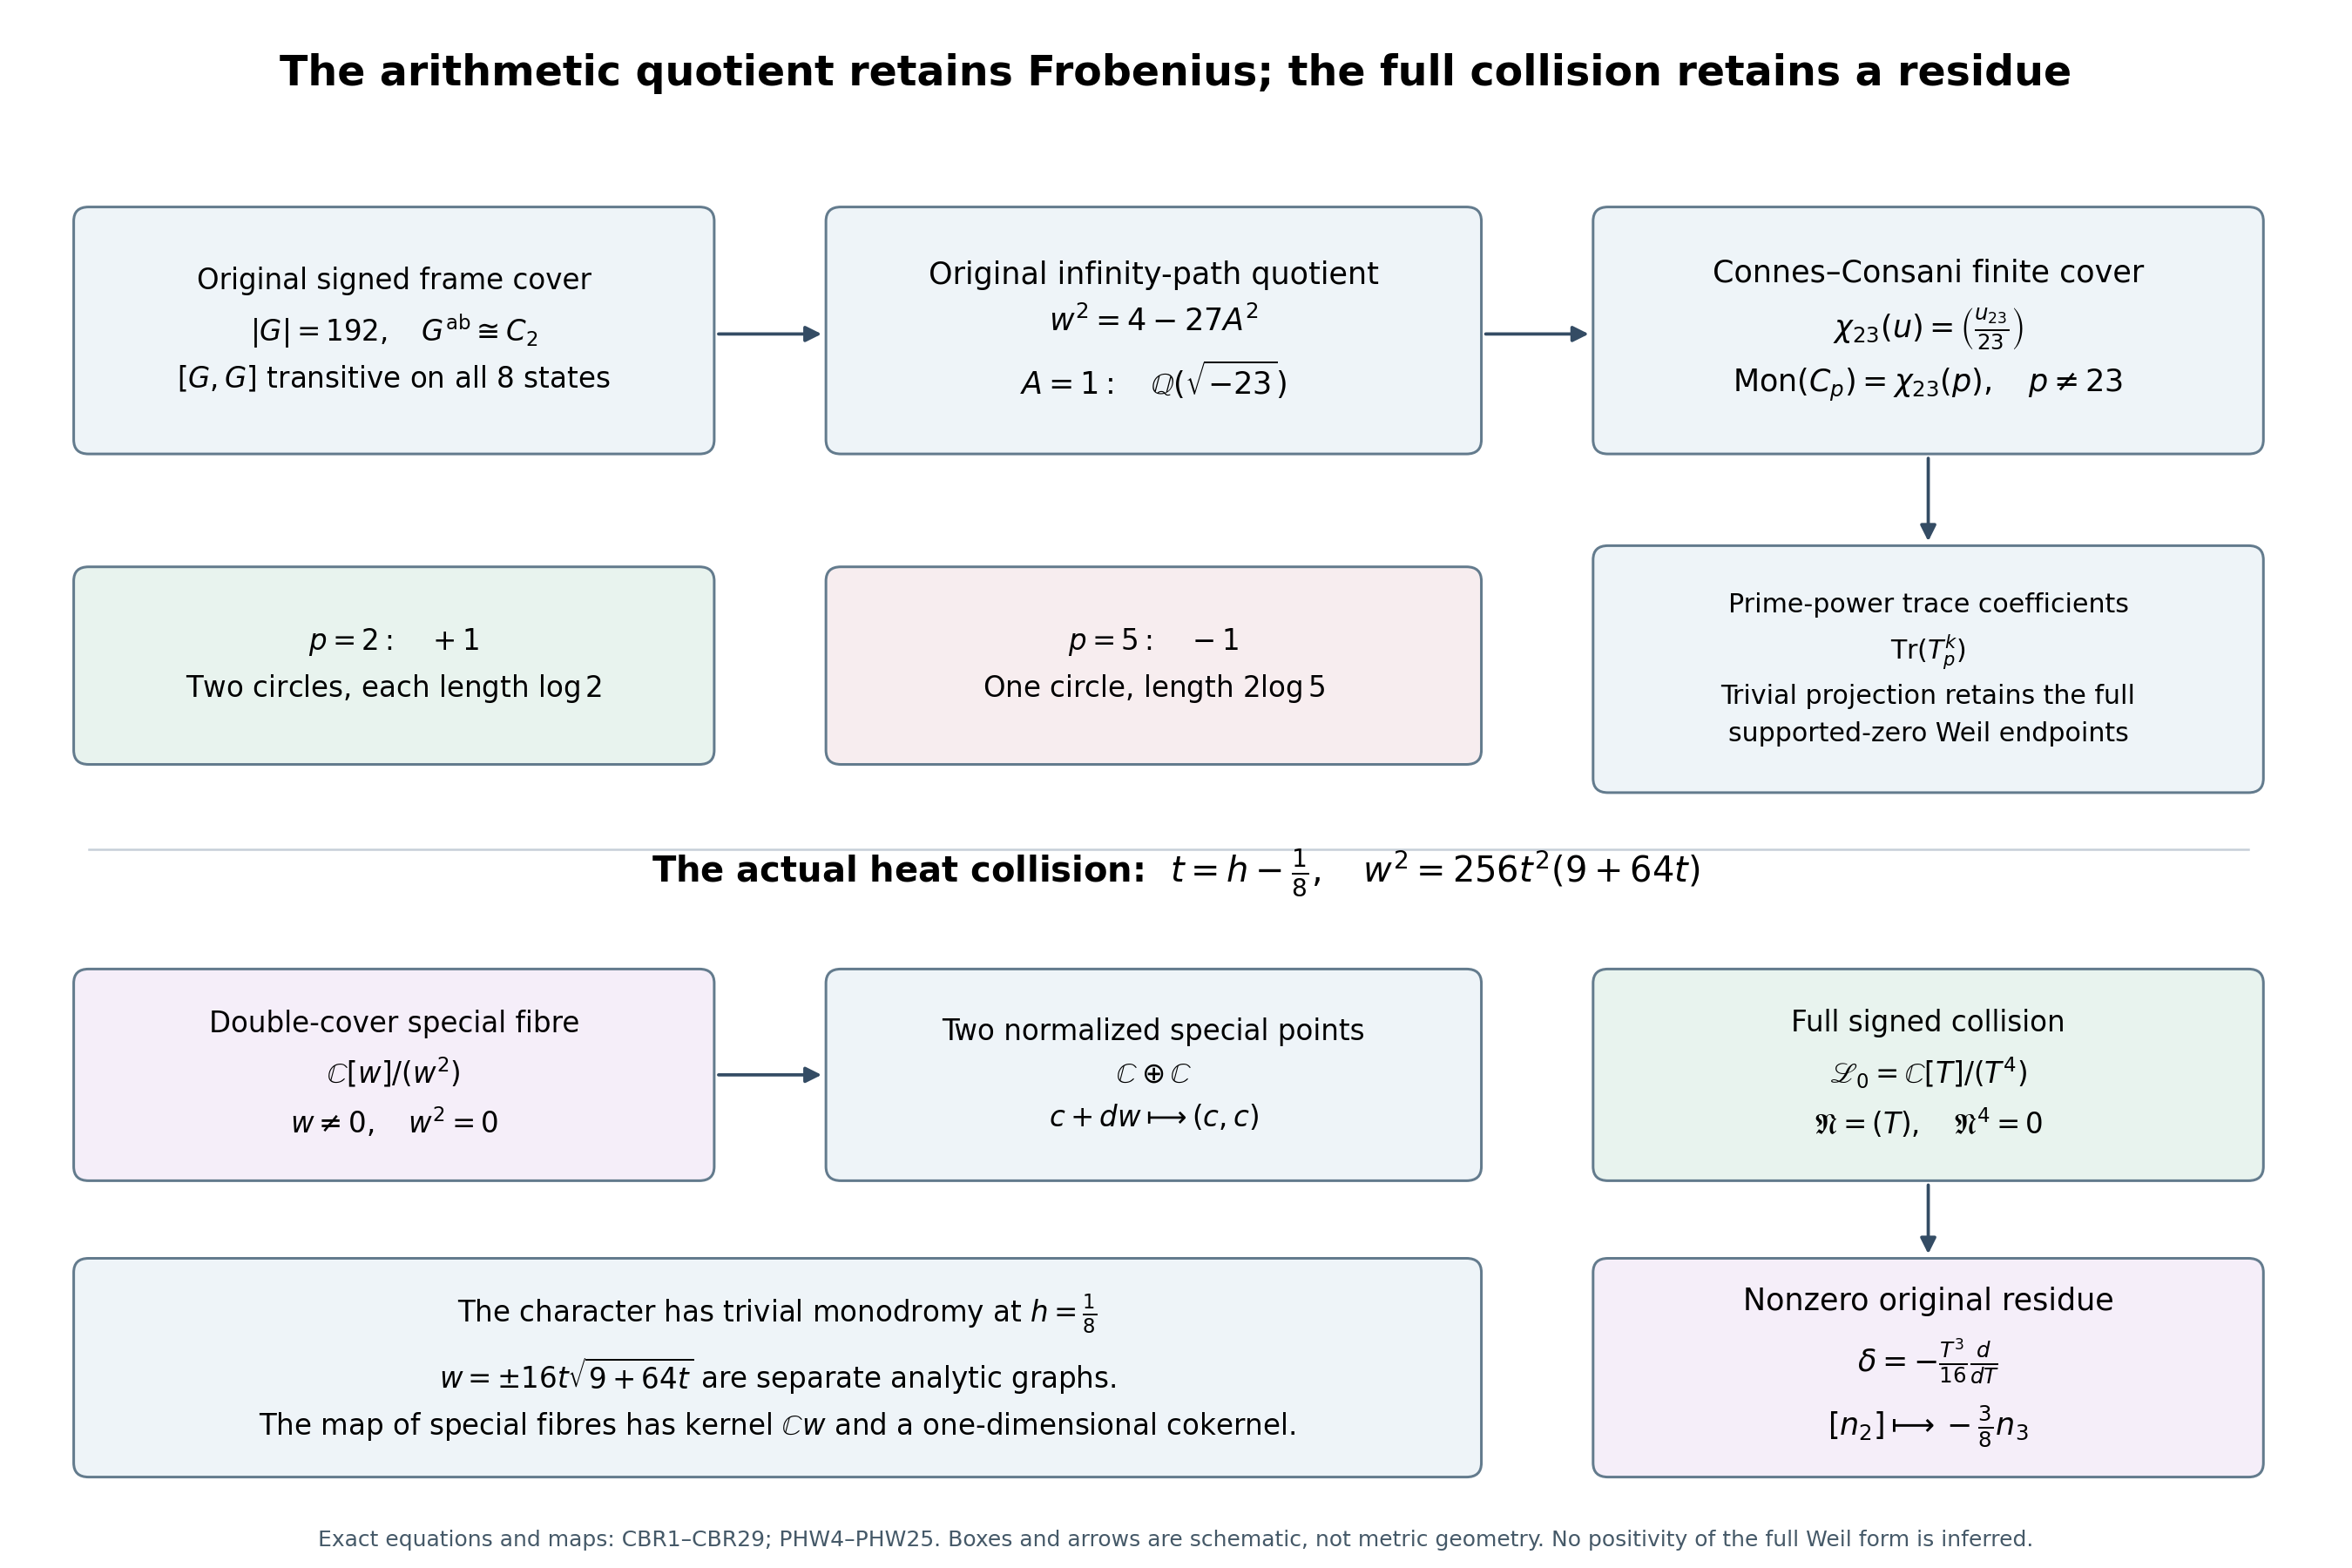
\includegraphics[keepaspectratio,alt={The original frame-cover quotient, its arithmetic specialization and prime returns, the two different special-fibre maps, and the surviving holonomy residue. CBR1--CBR29 and PHW4--PHW25 prove these exact maps. The box arrangement is schematic.}]{figures/34_class_field_holonomy.png}}
\caption{The original frame-cover quotient, its arithmetic
specialization and prime returns, the two different special-fibre maps,
and the surviving holonomy residue. CBR1--CBR29 and PHW4--PHW25 prove
these exact maps. The box arrangement is schematic.}
\end{figure}

\end{document}
